\documentclass[a4paper,10pt]{llncs}

%% There is a package that you should include first: nag. Why first? Because it warns you about
%% obsolete commands and package. https://daniel-j-h.github.io/post/latex-a-modern-approach/
\usepackage[l2tabu,orthodox]{nag}

\usepackage{ifxetex}

%% TYPOGRAPHY

\usepackage{microtype}
% uncomment to enable palatino
% \usepackage{palatino,mathpazo}

\usepackage[bookmarksdepth=2]{hyperref}

\usepackage{lineno}
\linenumbers{}

%% TODO NOTES

\usepackage{xcolor}
\definecolor{oxygenorange}{HTML}{FFDD00}
\usepackage[color=oxygenorange]{todonotes}
\newcommand{\malb}[2][inline]{\todo[#1]{\textbf{malb:} #2}\xspace}

%% ANONYMOUS SUBMISSIONS

\def\isanonymous{0}

\usepackage{ifthen}
\newcommand{\anonymous}[2]{
\ifthenelse{\equal{\isanonymous}{1}}
{{#1}}
{{#2}}
}

%% MATHEMATICAL SYMBOLS

\usepackage{amsmath,amsfonts,amssymb}
\usepackage{xspace}

%% CRYPTO Notation

\usepackage[lambda,landau,operators,probability,sets,logic,complexity,asymptotics]{cryptocode}

%% OTHER PACKAGES

\usepackage{booktabs}  %% tables
\usepackage{comment}
\usepackage{enumitem}

\ifxetex%
\else%
\usepackage{embedfile}
\fi%

%% PLOTS 

\usepackage{tikz,pgfplots}
\usetikzlibrary{calc}
\usetikzlibrary{arrows}

% from pgfplotsthemetol.sty
\definecolor{DarkPurple}{HTML}{332288}
\definecolor{DarkBlue}{HTML}{6699CC}
\definecolor{LightBlue}{HTML}{88CCEE}
\definecolor{DarkGreen}{HTML}{117733}
\definecolor{DarkRed}{HTML}{661100}
\definecolor{LightRed}{HTML}{CC6677}
\definecolor{LightPink}{HTML}{AA4466}
\definecolor{DarkPink}{HTML}{882255}
\definecolor{LightPurple}{HTML}{AA4499}

\definecolor{DarkBrown}{HTML}{604c38}
\definecolor{DarkTeal}{HTML}{23373b}
\definecolor{LightBrown}{HTML}{EB811B}
\definecolor{LightGreen}{HTML}{14B03D}

%% LISTINGS

\usepackage{listings}
\lstdefinelanguage{Sage}[]{Python}{morekeywords={True,False,sage,cdef,cpdef,ctypedef,self},sensitive=true}
\lstset{frame=none,
          showtabs=False,
          showspaces=False,
          showstringspaces=False,
          commentstyle=\color{gray!80!black},
          keywordstyle={\color{gray!80!black}\textbf},
          stringstyle ={\color{gray!80!black}},
          % frame=single,
          basicstyle=\tt\small\relax,,
          }


%% OPENING

\title{A well-written paper about interesting stuff}
\anonymous{}{\author{Martin R. Albrecht}}

\begin{document}

\maketitle

\begin{abstract}
  We do stuff.
\end{abstract}

\section{Introduction}\label{sec:introduction}

\malb{An example note for some example text.}

Several improvements of BKZ have been suggested and their combination is often referred to as BKZ 2.0~\cite{AC:CheNgu11}. These improvements are extreme pruning~\cite{EC:GamNguReg10}, early termination, limiting the enumeration radius to the Gaussian Heuristic and local block pre-processing. Extreme pruning takes place in the enumeration subroutine, and it works by exploring only certain branches in the search tree, with the hope that a short enough vector is still found, therefore decreasing the runtime. Early termination is based on the observation that the quality of the output basis increases more dramatically in the earlier rounds of BKZ\@. Therefore, continuing to reduce the lattice offers diminishing returns in the basis quality, and early termination decreases the runtime while still returning a basis close to the desired quality. Local block pre-processing takes the form of running BKZ-$k'$ with early termination for some value $k'$ so that the local basis is more than merely LLL reduced.

\subsubsection{Quality of Output.} Assuming that the Gaussian Heuristic (GH) and the \emph{Geometric Series Assumption} (GSA) hold for a lattice, Chen\malb[]{Cite PhD thesis} gives a limiting value of the root-Hermite factor $\delta_0$ achievable by BKZ as a function of the block size $k$:

\begin{equation}\label{eq:k-delta}
\lim_{n \rightarrow \infty} \delta_0 ={\left(v_k^{\frac{-1}{k}}\right)}^{\frac{1}{k-1}}  \approx  {\left( \frac{k}{2 \pi e} {(\pi k)}^{\frac{1}{k}}  \right)}^{\frac{1}{2(k-1)}}
\end{equation}
where $v_k$ is the volume of the unit ball in dimension $k$. Experimental evidence suggests that we may apply the right hand side of~\eqref{eq:k-delta} as an estimate for $\delta_0$ also when $n$ is finite.

The `lattice rule of thumb' is often used to given an approximation for  $\delta_0$ for a given $k$ as $\delta_0 = k^{\frac{1}{2k}}$. To ease analysis, this expression, in turn, is often approximated by $\delta_0 = 2^{1/k}$.

We note that depending on which estimate is used vastly different relations between $k$ and $\delta_0$ are assumed. To illustrate this we plot predictions for $\delta_0$ for block sizes $50 \leq k \leq 250$ in Figure~\ref{fig:delta-blocksize}.

\begin{figure}[ht]
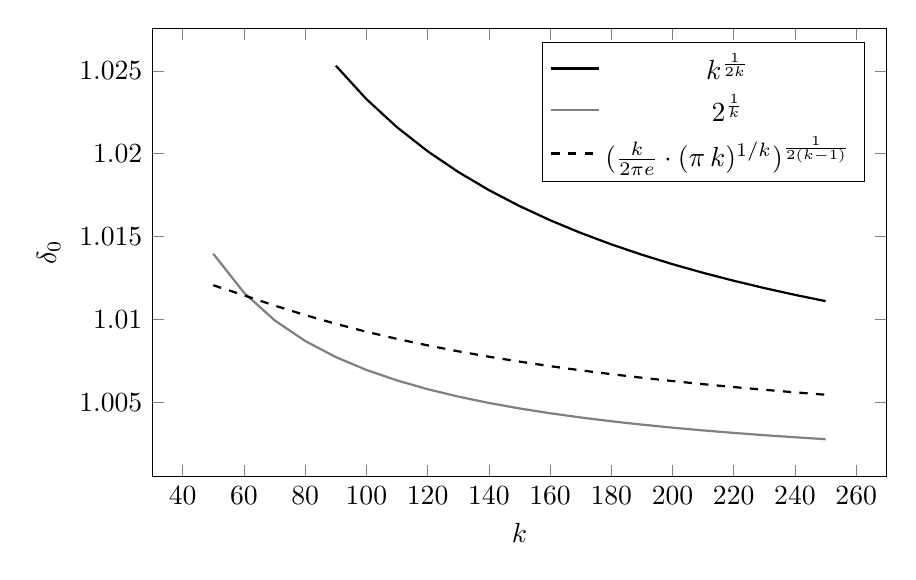
\begin{tikzpicture}
\pgfplotsset{width=0.9\textwidth, height=0.6\textwidth}

\begin{axis}[xlabel={$k$},ylabel={$\delta_0$},legend pos=north east, legend style={fill=none},  yticklabel style={/pgf/number format/fixed, /pgf/number format/precision=4}]
\addplot[black, thick] coordinates {
(90, 1.02531403637007) 
(100, 1.02329299228075) (110, 1.02159570327009) (120, 1.02014817082573) (130, 1.01889762835997) (140, 1.01780538190175) (150, 1.01684237780642) (160, 1.01598635421221) (170, 1.01521995101070) (180, 1.01452942078216) (190, 1.01390372822689) (200, 1.01333390755540) (210, 1.01281259525780) (220, 1.01233368464143) (230, 1.01189206652013) (240, 1.01148343189850) (250, 1.01110411995830)
};

\addlegendentry{$k^{\frac{1}{2k}}$};
\addplot[gray, thick] coordinates {
(50, 1.01395947979003) (60, 1.01161944030192) (70, 1.00995129061812)
(80, 1.00870198379040) (90, 1.00773136921715) (100, 1.00695555005672)
(110, 1.00632123320225) (120, 1.00579294106785) (130, 1.00534614127244)
(140, 1.00496332799666) (150, 1.00463167440205) (160, 1.00434156729192)
(170, 1.00408566000104) (180, 1.00385824159448) (190, 1.00365480562900)
(200, 1.00347174850950) (210, 1.00330615417116) (220, 1.00315563757687)
(230, 1.00301822910283) (240, 1.00289228786937) (250, 1.00277643590108)
};
\addlegendentry{$2^{\frac{1}{k}}$};
         	
\addplot[black, thick,style=dashed] coordinates {
(50, 1.01206486355485) (60, 1.01145310214785) (70, 1.01083849117278)
(80, 1.01026264533039) (90, 1.00973613406057) (100, 1.00925872103633)
(110, 1.00882653150498) (120, 1.00843474281592) (130, 1.00807860284815)
(140, 1.00775378902354) (150, 1.00745650119215) (160, 1.00718344897388)
(170, 1.00693180103572) (180, 1.00669912477197) (190, 1.00648332800111)
(200, 1.00628260691082) (210, 1.00609540127612) (220, 1.00592035664374)
(230, 1.00575629268952) (240, 1.00560217684407) (250, 1.00545710232739)
};
\addlegendentry{$(\frac{k}{2\pi e} \cdot (\pi\, k)^{1/k} )^{\frac{1}{2(k-1)}}$};

% \addplot[gray, thick,style=dashed] coordinates {
% (  50,  1.0120434) (  60,  1.0114350) (  70,  1.0108255) (  80,  1.0102559) (  90,  1.0097365) ( 100,  1.0092670) ( 110,  1.0088426) ( 120,  1.0084601) ( 130,  1.0081140) ( 140,  1.0077959) ( 150,  1.0075077) ( 160,  1.0072485) ( 170,  1.0070125) ( 180,  1.0067926) ( 190,  1.0065821) ( 200,  1.0063746) ( 210,  1.0061897) ( 220,  1.0060298) ( 230,  1.0058886) ( 240,  1.0057615) ( 250,  1.0056449)
% };
%  \addlegendentry{BKZ sim.\ ($n=390$)};
\end{axis}
\end{tikzpicture}
\caption{Estimates for $\delta_0$ for BKZ-$k$.}\label{fig:delta-blocksize}
\end{figure}

\section{Source Code}

\begin{lstlisting}[language=C]
#include <stdio.h>
int main(int argc, char **argv) {
  printf("hello world\n"); // print
  exit(0);
}
\end{lstlisting}

\clearpage
\bibliographystyle{alpha}
\bibliography{cryptobib/abbrev3,cryptobib/crypto_crossref,local}

\end{document}

%%% Local Variables:
%%% mode: latex
%%% TeX-master: t
%%% End:
%%% chktex 17